\documentclass[border=6pt]{standalone}
\usepackage{fontspec,unicode-math}
\setmainfont{Noto Serif}
\setmathfont{STIXTwoMath-Regular.otf}
\usepackage{tikz}
\usetikzlibrary{arrows.meta,calc,patterns,decorations.markings,decorations.pathmorphing,decorations.pathreplacing}
\tikzset{lev/.style={line width=1.2pt,line cap=butt},
 fine/.style={line width=.54pt},light/.style={line width=.37pt},
 curve/.style={line width=1.2pt,line cap=round,line join=round},
 ax/.style={line width=.62pt,-{Latex[length=2.1mm,width=1.15mm]}},
 ray/.style={line width=.58pt,-{Latex[length=1.85mm,width=.95mm]},shorten >=1.4pt,shorten <=1.4pt},
 dim/.style={line width=.52pt,{Latex[length=1.6mm,width=.85mm]}-{Latex[length=1.6mm,width=.85mm]}},
 flow/.style={line width=.60pt,postaction={decorate},decoration={markings,mark=at position .62 with {\arrow{Latex[length=1.8mm,width=.95mm]}}}},
 lab/.style={font=\fontsize{12}{14.4}\selectfont,inner sep=1.6pt},
 small/.style={font=\fontsize{10.5}{12.5}\selectfont,inner sep=1.3pt},
 tinylabel/.style={font=\fontsize{9.2}{11}\selectfont,inner sep=1.0pt},
 panel/.style={font=\fontsize{12}{14.4}\selectfont\itshape,inner sep=1.5pt}}
\pagestyle{empty}
\begin{document}
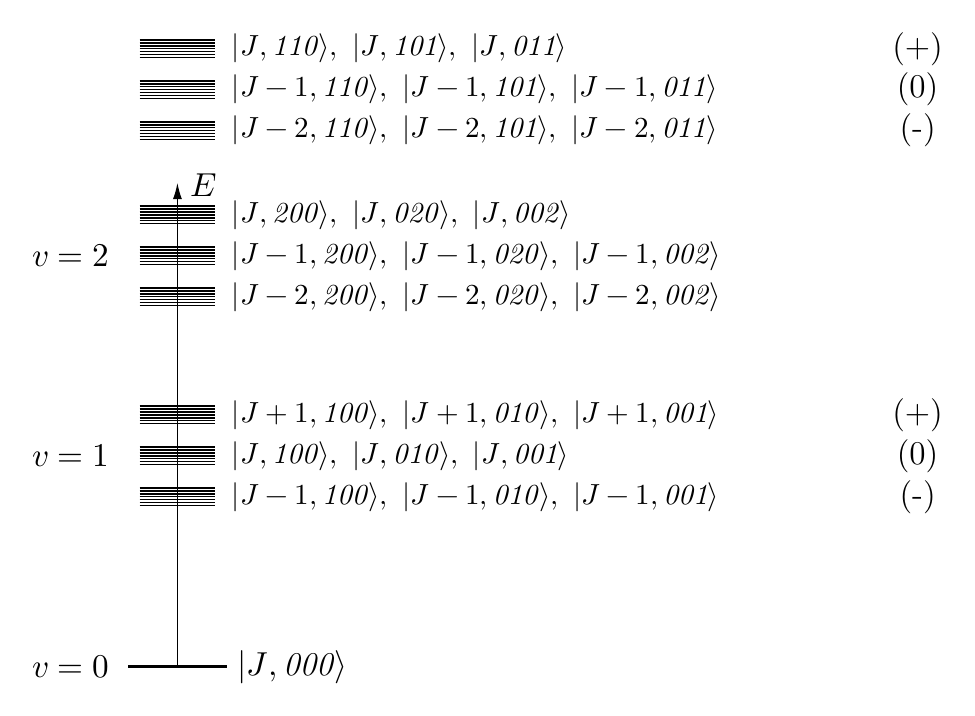
\begin{tikzpicture}[x=1cm,y=1cm,line join=round]
\coordinate (g) at (1.35000,0.00000);
\draw[lev] (0.72600,0.00000)--(1.97400,0.00000);
\node[lab,anchor=west] at (2.04400,0.00000) {$|J,\mathit{000}\rangle$};
\node[lab,anchor=east] at (0.55000,0.00000) {$v=0$};
\coordinate (v11) at (1.35000,3.20000);
\draw[fine] (0.87000,3.08900)--(1.83000,3.08900);
\draw[fine] (0.87000,3.12600)--(1.83000,3.12600);
\draw[fine] (0.87000,3.16300)--(1.83000,3.16300);
\draw[fine] (0.87000,3.20000)--(1.83000,3.20000);
\draw[fine] (0.87000,3.23700)--(1.83000,3.23700);
\draw[fine] (0.87000,3.27400)--(1.83000,3.27400);
\draw[fine] (0.87000,3.31100)--(1.83000,3.31100);
\node[small,anchor=west] at (1.99000,3.20000) {$|J+1,\mathit{100}\rangle,\ |J+1,\mathit{010}\rangle,\ |J+1,\mathit{001}\rangle$};
\node[lab] at (10.75000,3.20000) {(+)};
\coordinate (v10) at (1.35000,2.68000);
\draw[fine] (0.87000,2.56900)--(1.83000,2.56900);
\draw[fine] (0.87000,2.60600)--(1.83000,2.60600);
\draw[fine] (0.87000,2.64300)--(1.83000,2.64300);
\draw[fine] (0.87000,2.68000)--(1.83000,2.68000);
\draw[fine] (0.87000,2.71700)--(1.83000,2.71700);
\draw[fine] (0.87000,2.75400)--(1.83000,2.75400);
\draw[fine] (0.87000,2.79100)--(1.83000,2.79100);
\node[small,anchor=west] at (1.99000,2.68000) {$|J,\mathit{100}\rangle,\ |J,\mathit{010}\rangle,\ |J,\mathit{001}\rangle$};
\node[lab] at (10.75000,2.68000) {(0)};
\coordinate (v1m1) at (1.35000,2.16000);
\draw[fine] (0.87000,2.04900)--(1.83000,2.04900);
\draw[fine] (0.87000,2.08600)--(1.83000,2.08600);
\draw[fine] (0.87000,2.12300)--(1.83000,2.12300);
\draw[fine] (0.87000,2.16000)--(1.83000,2.16000);
\draw[fine] (0.87000,2.19700)--(1.83000,2.19700);
\draw[fine] (0.87000,2.23400)--(1.83000,2.23400);
\draw[fine] (0.87000,2.27100)--(1.83000,2.27100);
\node[small,anchor=west] at (1.99000,2.16000) {$|J-1,\mathit{100}\rangle,\ |J-1,\mathit{010}\rangle,\ |J-1,\mathit{001}\rangle$};
\node[lab] at (10.75000,2.16000) {(-)};
\node[lab,anchor=east] at (0.55000,2.68000) {$v=1$};
\coordinate (v2pure0) at (1.35000,5.74000);
\draw[fine] (0.87000,5.62900)--(1.83000,5.62900);
\draw[fine] (0.87000,5.66600)--(1.83000,5.66600);
\draw[fine] (0.87000,5.70300)--(1.83000,5.70300);
\draw[fine] (0.87000,5.74000)--(1.83000,5.74000);
\draw[fine] (0.87000,5.77700)--(1.83000,5.77700);
\draw[fine] (0.87000,5.81400)--(1.83000,5.81400);
\draw[fine] (0.87000,5.85100)--(1.83000,5.85100);
\node[small,anchor=west] at (1.99000,5.74000) {$|J,\mathit{200}\rangle,\ |J,\mathit{020}\rangle,\ |J,\mathit{002}\rangle$};
\coordinate (v2purem1) at (1.35000,5.22000);
\draw[fine] (0.87000,5.10900)--(1.83000,5.10900);
\draw[fine] (0.87000,5.14600)--(1.83000,5.14600);
\draw[fine] (0.87000,5.18300)--(1.83000,5.18300);
\draw[fine] (0.87000,5.22000)--(1.83000,5.22000);
\draw[fine] (0.87000,5.25700)--(1.83000,5.25700);
\draw[fine] (0.87000,5.29400)--(1.83000,5.29400);
\draw[fine] (0.87000,5.33100)--(1.83000,5.33100);
\node[small,anchor=west] at (1.99000,5.22000) {$|J-1,\mathit{200}\rangle,\ |J-1,\mathit{020}\rangle,\ |J-1,\mathit{002}\rangle$};
\coordinate (v2purem2) at (1.35000,4.70000);
\draw[fine] (0.87000,4.58900)--(1.83000,4.58900);
\draw[fine] (0.87000,4.62600)--(1.83000,4.62600);
\draw[fine] (0.87000,4.66300)--(1.83000,4.66300);
\draw[fine] (0.87000,4.70000)--(1.83000,4.70000);
\draw[fine] (0.87000,4.73700)--(1.83000,4.73700);
\draw[fine] (0.87000,4.77400)--(1.83000,4.77400);
\draw[fine] (0.87000,4.81100)--(1.83000,4.81100);
\node[small,anchor=west] at (1.99000,4.70000) {$|J-2,\mathit{200}\rangle,\ |J-2,\mathit{020}\rangle,\ |J-2,\mathit{002}\rangle$};
\node[lab,anchor=east] at (0.55000,5.22000) {$v=2$};
\coordinate (v2hyb0) at (1.35000,7.85000);
\draw[fine] (0.87000,7.73900)--(1.83000,7.73900);
\draw[fine] (0.87000,7.77600)--(1.83000,7.77600);
\draw[fine] (0.87000,7.81300)--(1.83000,7.81300);
\draw[fine] (0.87000,7.85000)--(1.83000,7.85000);
\draw[fine] (0.87000,7.88700)--(1.83000,7.88700);
\draw[fine] (0.87000,7.92400)--(1.83000,7.92400);
\draw[fine] (0.87000,7.96100)--(1.83000,7.96100);
\node[small,anchor=west] at (1.99000,7.85000) {$|J,\mathit{110}\rangle,\ |J,\mathit{101}\rangle,\ |J,\mathit{011}\rangle$};
\node[lab] at (10.75000,7.85000) {(+)};
\coordinate (v2hybm1) at (1.35000,7.33000);
\draw[fine] (0.87000,7.21900)--(1.83000,7.21900);
\draw[fine] (0.87000,7.25600)--(1.83000,7.25600);
\draw[fine] (0.87000,7.29300)--(1.83000,7.29300);
\draw[fine] (0.87000,7.33000)--(1.83000,7.33000);
\draw[fine] (0.87000,7.36700)--(1.83000,7.36700);
\draw[fine] (0.87000,7.40400)--(1.83000,7.40400);
\draw[fine] (0.87000,7.44100)--(1.83000,7.44100);
\node[small,anchor=west] at (1.99000,7.33000) {$|J-1,\mathit{110}\rangle,\ |J-1,\mathit{101}\rangle,\ |J-1,\mathit{011}\rangle$};
\node[lab] at (10.75000,7.33000) {(0)};
\coordinate (v2hybm2) at (1.35000,6.81000);
\draw[fine] (0.87000,6.69900)--(1.83000,6.69900);
\draw[fine] (0.87000,6.73600)--(1.83000,6.73600);
\draw[fine] (0.87000,6.77300)--(1.83000,6.77300);
\draw[fine] (0.87000,6.81000)--(1.83000,6.81000);
\draw[fine] (0.87000,6.84700)--(1.83000,6.84700);
\draw[fine] (0.87000,6.88400)--(1.83000,6.88400);
\draw[fine] (0.87000,6.92100)--(1.83000,6.92100);
\node[small,anchor=west] at (1.99000,6.81000) {$|J-2,\mathit{110}\rangle,\ |J-2,\mathit{101}\rangle,\ |J-2,\mathit{011}\rangle$};
\node[lab] at (10.75000,6.81000) {(-)};
\draw[ax] (1.35000,0.00000)--(1.35000,6.15000);
\node[lab,anchor=west] at (1.45000,6.12000) {$E$};
\end{tikzpicture}
\end{document}
